\documentclass[10pt,oneside]{article}

\usepackage[T1]{fontenc}
\usepackage{fontawesome}

\usepackage[paper=a4paper,margin=2cm,bottom=2.5cm]{geometry}
\usepackage[sfdefault,light,condensed]{roboto}
\usepackage[export]{adjustbox}
\usepackage[usenames,dvipsnames,table]{xcolor}

\usepackage{amsmath,amssymb,array,fancyhdr,graphicx,enumitem,lastpage,multicol,tabularx,textcomp,titlesec}
\usepackage{mathtools}

\setlength\extrarowheight{1pt}
\setlength\parindent{0cm}
\renewcommand\headrule{}
\setlength{\footskip}{1.25cm}

\pagestyle{fancy}

\definecolor{BoxHeaderBG}{RGB}{50, 50, 50}
\definecolor{BoxHeaderText}{RGB}{255, 255, 255}

\newcommand{\BoxHeader}[2]{
    \multicolumn{#1}{| >{\bfseries\footnotesize\cellcolor{BoxHeaderBG}\arraybackslash}l |}{
        \textcolor{BoxHeaderText}{#2}
    }
}

\definecolor{ATLHeaderBG}{RGB}{65, 190, 30}
\definecolor{ATLHeaderText}{RGB}{0, 0, 0}

\definecolor{ATLSkillBG}{RGB}{215, 230, 210}
\definecolor{ATLSkillText}{RGB}{0, 0, 0}

\definecolor{DefinitionBoxHeaderBG}{RGB}{30, 30, 110}
\definecolor{DefinitionBoxHeaderText}{RGB}{255, 255, 255}

\definecolor{FormativeHeaderBG}{RGB}{150, 30, 150}
\definecolor{FormativeHeaderText}{RGB}{255, 255, 255}

\definecolor{GlobalContextHeaderBG}{RGB}{255, 255, 150}
\definecolor{GlobalContextHeaderText}{RGB}{0, 0, 0}

\definecolor{KeyConceptHeaderBG}{RGB}{15, 225, 225}
\definecolor{KeyConceptHeaderText}{RGB}{0, 0, 0}

\definecolor{RelatedConceptHeaderBG}{RGB}{15, 170, 170}
\definecolor{RelatedConceptHeaderText}{RGB}{0, 0, 0}

\definecolor{QuestionHeaderBG}{RGB}{240, 240, 240}
\definecolor{QuestionHeaderText}{RGB}{0, 0, 0}

\definecolor{SolutionHeaderBG}{RGB}{225, 150, 110}
\definecolor{SolutionHeaderText}{RGB}{0, 0 , 0}

\definecolor{SummativeHeaderBG}{RGB}{195, 15, 15}
\definecolor{SummativeHeaderText}{RGB}{255, 255, 255}

\newcommand{\ATLHeader}[1]{
    \cellcolor{ATLHeaderBG}\textcolor{ATLHeaderText}{
        \bfseries\footnotesize
        ATL SKILL (#1) \hfill \faGears
    }
}

\newcommand{\ATLSkill}[1]{
    \cellcolor{ATLSkillBG}\textcolor{ATLSkillText}{
        \itshape #1
    }
}

\newcommand{\DefinitionBoxHeader}{
    \cellcolor{DefinitionBoxHeaderBG}\textcolor{DefinitionBoxHeaderText}{
        \bfseries\footnotesize
        DEFINITIONS \hfill \faPencil
    }
}

\newcommand{\FormativeHeader}{
    \cellcolor{FormativeHeaderBG}\textcolor{FormativeHeaderText}{
        \bfseries\footnotesize
        FORMATIVE ASSESSMENT \hfill \faComments
    }
}

\newcommand{\GlobalContextHeader}[1]{
    \cellcolor{GlobalContextHeaderBG}\textcolor{GlobalContextHeaderText}{
        \bfseries\footnotesize
        GLOBAL CONTEXT (#1) \hfill \faGlobe
    }
}

\newcommand{\KeyConceptHeader}[1]{
    \cellcolor{KeyConceptHeaderBG}\textcolor{KeyConceptHeaderText}{
        \bfseries\footnotesize
        KEY CONCEPT (#1) \hfill \faKey
    }
}

\newcommand{\RelatedConceptHeader}[1]{
    \cellcolor{RelatedConceptHeaderBG}\textcolor{RelatedConceptHeaderText}{
        \bfseries\footnotesize
        RELATED CONCEPT (#1) \hfill \faLink
    }
}

\newcommand{\SolutionHeader}[1]{
    \cellcolor{SolutionHeaderBG}\textcolor{SolutionHeaderText}{
        \bfseries\footnotesize 
        #1 \hfill \faPaste
    }
}

\newcommand{\SummativeHeader}{
    \cellcolor{SummativeHeaderBG}\textcolor{SummativeHeaderText}{
        \bfseries\footnotesize
        SUMMATIVE ASSESSMENT \hfill \faCheck
    }
}

\newcounter{QuestionCounter}

\newcommand{\QuestionBox}[1]{
    \stepcounter{QuestionCounter}
    \cellcolor{QuestionHeaderBG}\textcolor{QuestionHeaderText}{
        {\bfseries\scriptsize Q\theQuestionCounter} #1
    }
}

\newcommand{\boxwidth}{\linewidth}

\lhead{\scriptsize\texttt{U\UnitNumber: \UnitTitle \\ L\LessonNumber: \LessonTitle}}
\rhead{\scriptsize\ttfamily [DESIGN/\CourseName/U\UnitNumber/L\LessonNumber]\\\ }

\lfoot{
\includegraphics[height=2cm,valign=c]{Files/logo}}
\cfoot{\footnotesize DESIGN/\CourseName/U\UnitNumber/L\LessonNumber\ | \LessonTitle \\ Woodstock School | Mussoorie, Uttarakhand, India}
\rfoot{
\includegraphics[height=2cm,valign=c]{Files/ib-world-school-logo-1-colour}}

\titleformat{\section}{\normalfont\Large\bfseries}{}{0em}{}[{\titlerule[0.5pt]}]
\titleformat{\subsection}{\normalfont\large\bfseries}{}{0em}{}


\usepackage{circuitikz,subcaption,tikzsymbols}

\usetikzlibrary{arrows}

\def\CourseName{MYP3}

\def\LessonNumber{01}
\def\LessonTitle{Simple Circuits}

\def\UnitNumber{01}
\def\UnitTitle{Circuits \& Electronics}

\begin{document}
    \begin{center}
        \huge\bfseries
        \LessonTitle
    \end{center}

    \section{Before You Begin}

    Answer each of the following questions related to this unit's global context: \emph{Orientation in Space \& Time}.

    \medskip
    \begin{tabularx}{\boxwidth}{| X |}
        \hline
        \GlobalContextHeader{Orientation in Space \& Time}\\\hline
        \QuestionBox{Imagine you were living during a time \emph{without} electricity. How much of your current lifestyle would be different? How much would be the same?}\\\hline
        \ \\[5cm]\hline
        \QuestionBox{In what ways has access to electricity and electronic devices shaped who you are?}\\\hline
        \ \\[5cm]\hline
        \QuestionBox{The statement of inquiry for this unit is \emph{the invention of electricity and electronics was a turning point in the history of human development}. Do you agree with this statement? Why or why not?}\\\hline
        \ \\[5cm]\hline
    \end{tabularx}
    
    \pagebreak
 
    \section{Technical Background} 

    While a full understanding of electricity is beyond the scope of this course, a basic understanding of some terminology and components is required to understand the technical skills you will be developing. Below is a very simple overview to get us started.

    \subsection{Electrical Circuits}
 
    %TODO: Fix this "hack" for definition tables.
    \begin{tabularx}{\boxwidth}{| X |}
        \hline
        \DefinitionBoxHeader\\\hline
    \end{tabularx}

    \vspace*{-1pt}
    \begin{tabularx}{\boxwidth}{| >{\bfseries}p{0.15\boxwidth} | X |}
        Electrical Circuit & An \emph{electrical circuit} is any path from a \emph{source} of electricity to a \emph{ground}. \\\hline
        Source & A \emph{source} is anything that provides electrical energy, such as power plant, solar panels, or a battery. \\\hline
        Ground / Return & The \emph{ground} or \emph{return} in an electrical circuit is the destination for electrical energy.\\\hline
    \end{tabularx}


    \subsubsection*{Examples}
    Here are a few examples of common electrical circuits.

    \begin{figure}[h]
        \centering
        \begin{subfigure}[t]{0.45\boxwidth}
            \centering
            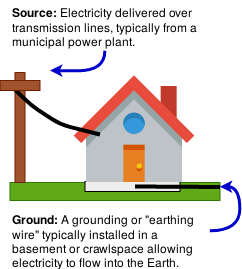
\includegraphics[height=6cm]{Extras/house_electricity}
            \caption*{A simple home electrical circuit.}
        \end{subfigure}
        \begin{subfigure}[t]{0.45\boxwidth}
            \centering
            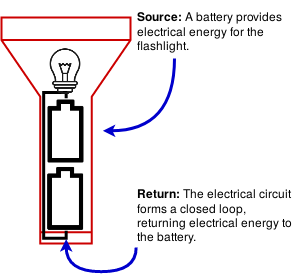
\includegraphics[height=6cm]{Extras/flashlight_electricity}
            \caption*{The electrical circuit in a flashlight.}
        \end{subfigure}
    \end{figure}

    Of course, electrical circuits are not that interesting if they don't \emph{do} anything. This is where the concept of a \emph{load} comes into play.

    \medskip
    \begin{tabularx}{\boxwidth}{| >{\bfseries}p{0.15\boxwidth} | X |}
        \hline
        Load & A \emph{load} in an electrical circuit is anything that consumes electrical energy to produce some result.\\\hline
    \end{tabularx}

    \bigskip
    \begin{tabularx}{\boxwidth}{| X | }
        \hline
        \ATLHeader{Communication Skills} \\\hline
        \ATLSkill{...make inferences and draw conclusions...} \\\hline
        \QuestionBox{{\scriptsize\bfseries Q1} Briefly describe the \emph{loads} typical to the two electrical circuits given above.} \\\hline
        \ \\[6cm]\hline
    \end{tabularx}

    \pagebreak
    \subsection{Simple Components}
    We are going to build a few simple circuits to explore electricity and its various applications. Here is a list of the components we will need for this first lesson.

    \medskip
    \begin{tabularx}{\boxwidth}{| >{\bfseries}p{0.15\boxwidth} | X | >{\centering\arraybackslash}p{0.15\boxwidth} | >{\centering\arraybackslash}p{0.15\boxwidth}| }
        \hline
        \BoxHeader{1}{Name} & \BoxHeader{1}{Description} & \BoxHeader{1}{Symbol} & \BoxHeader{1}{Example} \\\hline
        Coin Battery & A \emph{coin battery} works just like a battery you're probably already familiar with such as the typical AA or AAA batteries, except its shape resembles a coin. These batteries typically provide 3 volts of electrical energy. 
        
        \medskip
        The image on the right is of a common CR2032, named because it has a diameter of 20mm and a thickness of 3.2mm. & \raisebox{-1cm}{\tikz \draw(0, 0) node[below,xshift=20] {+} to [battery1] (2, 0);} & 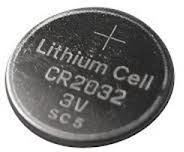
\includegraphics[width=0.9\boxwidth,valign=t]{Extras/coin_battery} \\\hline

        Light-Emitting Diode (LED) & A \emph{light-emitting diode}, or LED, is a typical light source in electronic circuits and many consumer devices. They are available in a wide variety of colours and sizes. The one shown on the right has a red lens with a diameter of 5mm. 
        
        \medskip
        Note that an LED only allows electricity to flow in one direction, noted by the arrow in the symbol and, typically, a flat side of the lens and shorter leg.
        & \raisebox{-1cm}{\tikz \draw(0, 0) to [full led] (2, 0);} & 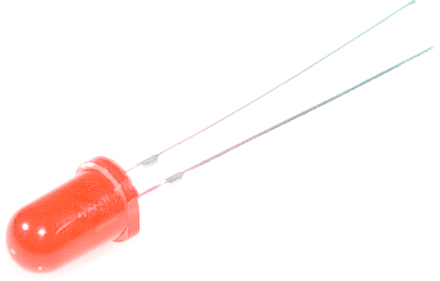
\includegraphics[width=0.9\boxwidth,valign=t]{Extras/led} \\\hline

        Push Button & A push button is a mechanical switch which ``closes'' or ``opens'' an electrical circuit. 
        
        \medskip
        The ones included in your electronics kit are ``normally-open, momentary'' push buttons. This means that if you don't press them, the electrical circuit is open (normally-open), and a spring forces the button to return to its default position after you release it (momentary). 
        & \raisebox{-1cm}{\tikz \draw(0, 0) to [push button] (2, 0);} & 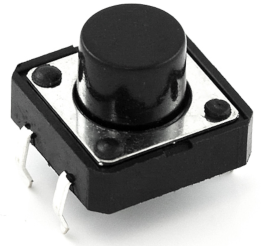
\includegraphics[width=0.9\boxwidth,valign=t]{Extras/pushbutton} \\\hline    
    \end{tabularx}
    
    \medskip
    Note that the symbols listed above will be useful when expressing circuits in circuit diagrams, explained below.

    \subsection{Circuit Diagrams}
    A circuit diagram uses symbols and lines to represent electrical circuits in a simplified way. Below is an example of a simple circuit diagram.

    \vspace*{1cm}

    \begin{minipage}{0.33\boxwidth}
        \begin{center}
            \begin{circuitikz}[scale=1.25]
                \draw(0, 1) node[left,yshift=-6] {+} to [battery1] (0, 0); 
                \draw(0, 1) to (0, 2) to (1, 2) to [push button] (2, 2)  to (3, 2) to  (3, 1) to [full led] (3, 0) to (3, -1) to (0, -1) to (0, 0);
            \end{circuitikz}
        \end{center}
    \end{minipage}
    \begin{minipage}{0.05\boxwidth}
        \ 
    \end{minipage}
    \begin{minipage}{0.6\boxwidth}
        \begin{center}
            \begin{tabularx}{\boxwidth}{| X | }
                \hline
                \ATLHeader{Communication Skills} \\\hline
                \ATLSkill{...use and interpret a range of discipline-specific terms and symbols...} \\\hline
                \QuestionBox{{\scriptsize\bfseries Q2} Identify and label each of the components in the diagram on the left.} \\\hline
                \QuestionBox{{\scriptsize\bfseries Q3} What do the lines show in a circuit diagram?} \\\hline
                \ \\[1.75cm]\hline
            \end{tabularx}
        \end{center}
    \end{minipage}

    \vspace*{1cm}

    \textbf{Note:} You might have learned in Physics class that electricity is the flow of electrons from a source of negative potential to positive. This is called the ``electron flow'' model of electricity. However, this is an understanding of physics that is \emph{newer} than the study of electrical circuits. In ``conventional flow'', we think of electricity as flowing from positive to negative.

    \medskip
    All of the circuit diagrams you see in this course, as well as a majority of diagrams you'll find elsewhere, are written under the conventional flow assumption. 

    \pagebreak

    \section{Developing Technical Skills}
    We will begin our exploration of electrical circuits by building \emph{paper circuits}. These circuits are built by using conductive tape (typically a copper foil) placed on paper with other components placed appropriately on top of this tape and secured using normal cellophane tape.

    \subsection{Circuit \#1}
    This is the simplest circuit we will work with, but will allow you to practice using the available materials for building paper circuits.

    \subsubsection*{You Will Need:}
    \begin{itemize}[noitemsep]\small
        \item (1) CR2032 Coin Battery
        \item (1) LED
        \item (1) Roll of Copper Tape
        \item (1) Roll of Cellophane Tape
    \end{itemize}

    \subsubsection*{Directions:}
    Create the paper circuit below by tracing the lines with copper tape and placing the components where indicated.

    \medskip
    \textbf{Note:} For a coin battery, the positive and negative terminals are the top and bottom of the battery. This requires the battery to be ``sandwiched'' between the copper tape as indicated in the diagram below.

    \begin{center}
        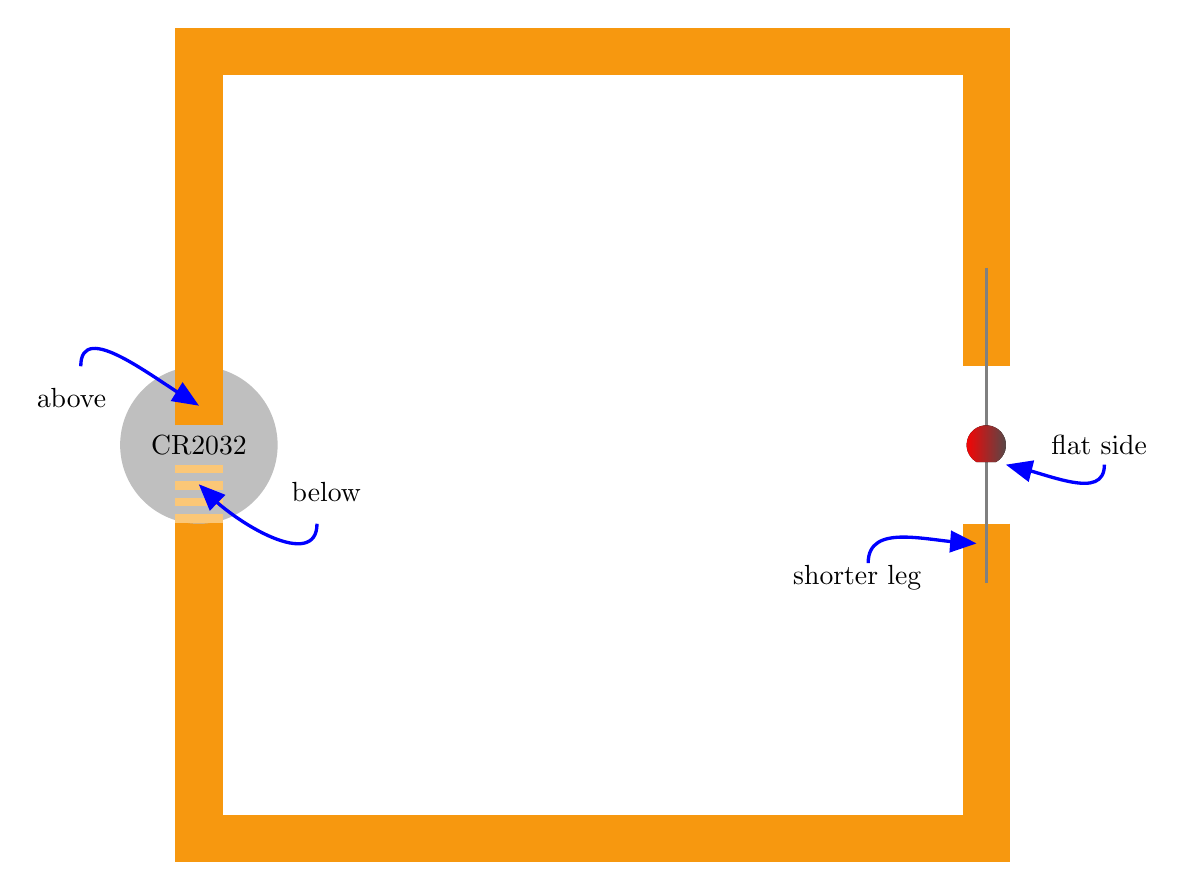
\begin{tikzpicture}
            \draw[line width=6mm,YellowOrange] (0, 0) -- (0, 5) -- (10, 5) -- (10, 1);
            \draw[line width=6mm,YellowOrange] (10, -1) -- (10, -5) -- (0, -5) -- (0, 0);

            \fill[black!25] (0, 0) circle (10mm);            
            \draw[line width=6mm, dashed,YellowOrange!50] (0, -0.25) -- (0, -1);
            \draw[line width=6mm,YellowOrange] (0, 0.25) -- (0, 1);
            \node[align=center] at (0, 0) {CR2032};

            \draw[very thick,black!50] (10, 2.25) -- (10, -1.75);
            \fill[left color=red, right color=black!70] ([shift=(-60:2.5mm)]10,0) arc (-60:240:2.5mm);

            \node[anchor=south east, xshift=-30, yshift=10] at (0, 0) {above};
            \draw[->,>=triangle 45,blue,very thick] (-1.5, 1) to [out=90,in=150] (0, 0.5);
            \node[anchor=north west, xshift=30, yshift=-10] at (0, 0) {below};
            \draw[->,>=triangle 45,blue,very thick] (1.5, -1) to [out=-90,in=-50] (0, -0.5);
            
            \node[align=left,anchor=west,xshift=20] at (10, 0) {flat side};
            \node[anchor=north east,xshift=-20,yshift=-40] at (10, 0) {shorter leg};
            \draw[->,>=triangle 45,blue,very thick] (11.5, -0.25) to [out=-90, in=-10] (10.25, -0.25);
            \draw[->,>=triangle 45,blue,very thick] (8.5, -1.5) to [out=90,in=-180] (9.875, -1.25);
        \end{tikzpicture}
    \end{center}

    \pagebreak
    \subsection{Circuit \#2}
    This second circuit introduces some control over the flow of electricity by adding a push button.

    \subsubsection*{You Will Need:}
        \begin{itemize}[noitemsep]\small
            \item (1) CR2032 Coin Battery
            \item (1) LED
            \item (1) Push Button
            \item (1) Roll of Copper Tape
        \end{itemize}

    \subsubsection*{Directions}
    Create the following paper circuit. Your push button may look slightly different from the one in the diagram, so make the appropriate adjustments, particularly to the size of the gap where the button is placed.

    \begin{center}
        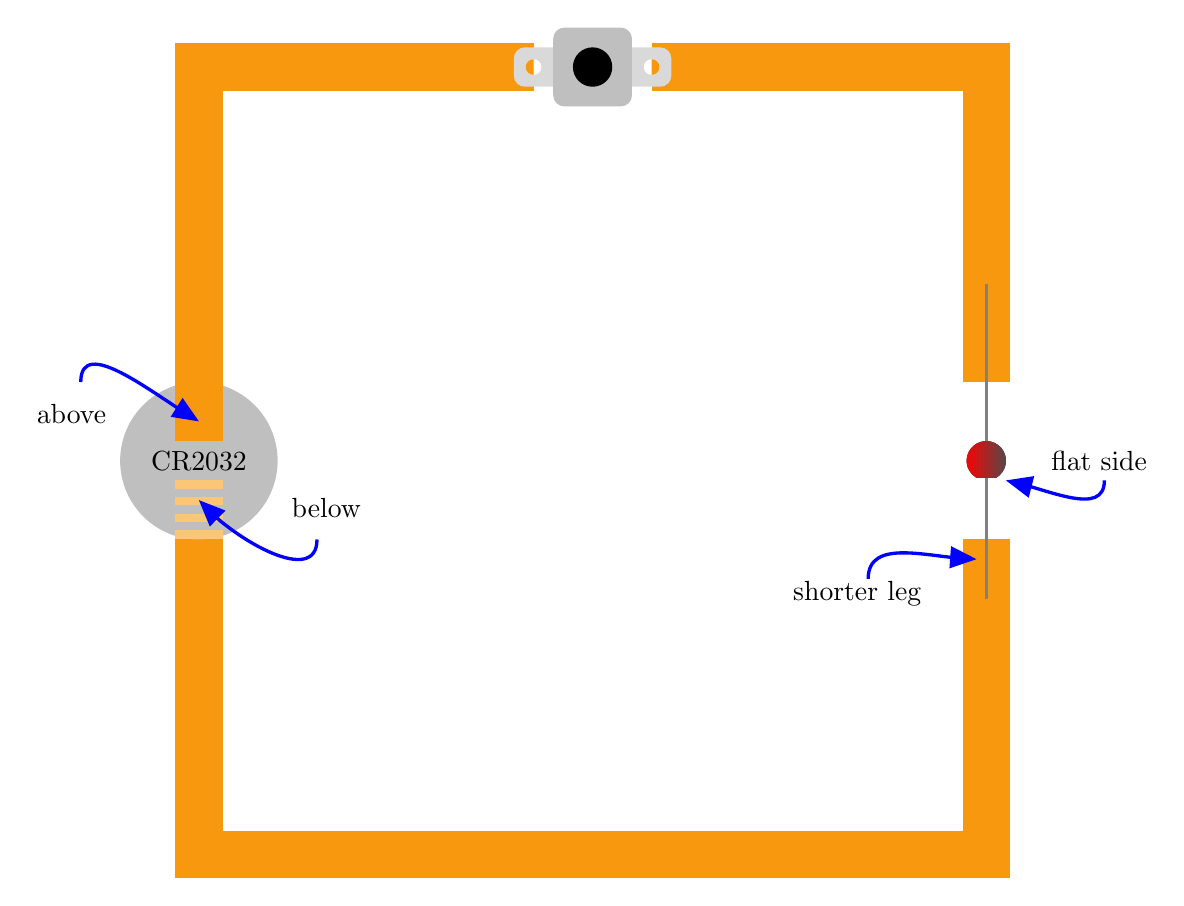
\begin{tikzpicture}
            \draw[line width=6mm,YellowOrange] (0, 0) -- (0, 5) -- (4.25, 5);
            \draw[line width=6mm,YellowOrange] (5.75, 5) -- (10, 5) -- (10, 1);
            \draw[line width=6mm,YellowOrange] (10, -1) -- (10, -5) -- (0, -5) -- (0, 0);

            \fill[black!25] (0, 0) circle (10mm);            
            \draw[line width=6mm, dashed,YellowOrange!50] (0, -0.25) -- (0, -1);
            \draw[line width=6mm,YellowOrange] (0, 0.25) -- (0, 1);
            \node[align=center] at (0, 0) {CR2032};

            \draw[very thick,black!50] (10, 2.25) -- (10, -1.75);
            \fill[left color=red, right color=black!70] ([shift=(-60:2.5mm)]10,0) arc (-60:240:2.5mm);

            \node[anchor=south east, xshift=-30, yshift=10] at (0, 0) {above};
            \draw[->,>=triangle 45,blue,very thick] (-1.5, 1) to [out=90,in=150] (0, 0.5);
            \node[anchor=north west, xshift=30, yshift=-10] at (0, 0) {below};
            \draw[->,>=triangle 45,blue,very thick] (1.5, -1) to [out=-90,in=-50] (0, -0.5);
            
            \node[align=left,anchor=west,xshift=20] at (10, 0) {flat side};
            \node[anchor=north east,xshift=-20,yshift=-40] at (10, 0) {shorter leg};
            \draw[->,>=triangle 45,blue,very thick] (11.5, -0.25) to [out=-90, in=-10] (10.25, -0.25);
            \draw[->,>=triangle 45,blue,very thick] (8.5, -1.5) to [out=90,in=-180] (9.875, -1.25);

            \fill[rounded corners,black!15] (4, 4.75) rectangle (6, 5.25);
            \fill[rounded corners,black!25] (4.5, 4.5) rectangle (5.5, 5.5);
            \fill[black] (5, 5) circle (0.25);
            \fill[white] (4.25, 5) circle (0.1);
            \fill[white] (5.75, 5) circle (0.1);
            \fill[YellowOrange] ([shift=(90:1mm)]4.25, 5) arc (90:270:1mm);
            \fill[YellowOrange] ([shift=(90:1mm)]5.75, 5) arc (90:-90:1mm);
        \end{tikzpicture}
    \end{center}

    \vspace{1cm}

    \begin{tabularx}{\boxwidth}{| X | }
        \hline
        \FormativeHeader \\\hline
        \QuestionBox{{\scriptsize\bfseries Q4} In the spaces below, sketch the circuit diagrams for each of the two paper circuits you built.} \\\hline
    \end{tabularx}

    \vspace*{-1pt}
    \begin{tabularx}{\boxwidth}{| X | X |}
        \hline
        \BoxHeader{1}{Circuit \#1} & \BoxHeader{1}{Circuit \#2}\\\hline
        \ & \ \\[4.5cm]\hline
    \end{tabularx}
    
    \pagebreak

    \begin{tabularx}{\boxwidth}{| X | }
        \hline
        \FormativeHeader \\\hline
        \QuestionBox{{\scriptsize\bfseries Q5} In the space below, sketch a paper circuit that will include (2) LEDs.} \\\hline
        \ \\[12cm]\hline
        \QuestionBox{{\scriptsize\bfseries Q6} Predict what will happen when your circuit is powered. Then, test your hypothesis by building the paper circuit.}
        \ \\\hline
        \ \\[4cm]\hline
        \QuestionBox{{\scriptsize\bfseries Q7} What actually happens when your circuit is powered? Why do you think this behaviour occurs?} \\\hline
        \ \\[4cm]\hline
    \end{tabularx}

    \pagebreak

    \section{Reflections}

    \begin{tabularx}{\boxwidth}{| X |}
        \hline
        \ATLHeader{Communication Skills}\\\hline
        \ATLSkill{...make inferences and draw conclusions...}\\\hline
        \QuestionBox{{\scriptsize\bfseries Q8} Why do you think the ability to draw conclusions from incomplete information or knowledge is an important skill to develop? Are there any dangers in doing so?}\\\hline
        \ \\[3.5cm]\hline
        \ATLSkill{...use and interpret a range of discipline-specific terms and symbols...}\\\hline
        \QuestionBox{{\scriptsize\bfseries Q9} In what other contexts are special terms and symbols used? Consider examples from your daily life, such as your hobbies and other activities, and not just academics.}\\\hline
        \ \\[3.5cm]\hline
    \end{tabularx}

    \bigskip
    \begin{tabularx}{\boxwidth}{| X |}
        \hline
        \QuestionBox{{\scriptsize\bfseries Q10} What aspect of this lesson was the most challenging for you? How did you overcome that challenge?}\\\hline
        \ \\[3.5cm]\hline
        \QuestionBox{{\scriptsize\bfseries Q11} Select the option which best reflects how confident you are in applying what you have learend in this lesson.}\\\hline
        \, \hfill \Sadey[5][orange] \hfill \Neutrey[5][gray] \hfill \Smiley[5][cyan] \hfill \,\\\hline
        \QuestionBox{{\scriptsize\bfseries Q12} What additional questions do you still have about this lesson's content?}\\\hline
        \ \\[3.5cm]\hline
    \end{tabularx}
\end{document}